\subsection{Множества и операции над ними. Булевы функции, КНФ, ДНФ. Базисы, теорема Поста.}

\subsubsection{Множества и операции над ними}

\subsubsection{Булевы функции, КНФ, ДНФ}
\T{В ДНФ можно выразить любую функцию}
\begin{proof}
	Рассмотрим строчки таблицы истинности с 1, для каждой напишем клоз из $n$ лиетралов, который выполняет ровно эту строчку.
	
	Википедия чета пишет про то, что тождественный 0 нельзя представить. Вообще можно, если можно писать $x \wedge \neg x$
\end{proof}

\T{В КНФ можно выразить любую булеву функцию}
\begin{proof}
	Построим ДНФ к отрицанию, повесим отрицание, по де-Моргану получим КНФ 
\end{proof}

\subsubsection{Базисы, теорема Поста}

Хуеста, блять, как же я затрахался. 

Булевы функции можно получать из других при помощи композиции. Возникает естественный вопрос, какими наборами функций можно выразить любую функцию.

\D{
	Стрелка Пирса: $x \uparrow y = \neg (x \vee y)$ 
}
\T{
	Стрелка Пирса - полный базис
}
\begin{proof}
	Получим конъюнкцию, дизъюнкцию и отрицание
	\begin{enumerate}
		\item $\neg x = x \uparrow x$
		\item $x \vee y = \neg (x \uparrow y)$
		\item $x \wedge y = \neq (\neg x \vee \neq y)$
	\end{enumerate}
\end{proof}

Вот Пост придумал критерий, как по набору функций понять, является ли он полным.

\textit{Замыкание класса функций} - это множество всех их возможных композиций.

Мы предъявляем 5 классов функций:
\begin{align*}
	T_0 = \{f \mid f(\overline{0}) = 0\}\\
	T_1 = \{f \mid f(\overline{1}) = 1\}\\
	M = \{f \mid \forall \alpha, \beta \in \mathbb{B}^n\ (\alpha \geq \beta) \rightarrow f(\alpha) \geq f(\beta)\}\\
	S = \{f \mid \forall \alpha \in \mathbb{B}^n f(\alpha) = \overline{f(\overline{\alpha})}\}\\
	L = \{f \mid f(x_1, x_2, \ldots x_n) = \alpha_0 \oplus \alpha_1x_1 \oplus \ldots \oplus \alpha_nx_n\}
\end{align*}

\T[Критерий поста]{
	Множество функций $F$ полно тогда и только тогда, когда в нем (его замыкании относительно композиций) есть функция, не принадлежащая ни одному из классов выше.
}

\begin{proof}
	Понятно, что если замыкание $F$ содержится в одном из классов, то $F$ не полно, т.к. ни один из классов не совпадает со множеством всех функций.
	
	В другую сторону докажем, что в $F$ можно реализовать конъюнкцию дизъюнкцию и отрицание. 
	
	\begin{figure}[H]
		\centering
		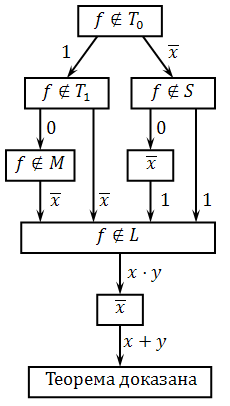
\includegraphics[scale=0.4]{images/post_sheme.png}
		\caption{Порядок перебора вариантов при доказательстве критерия Поста}
	\end{figure}
	
	Полное доказательство на \href{https://ru.wikipedia.org/wiki/%D0%9A%D1%80%D0%B8%D1%82%D0%B5%D1%80%D0%B8%D0%B9_%D0%9F%D0%BE%D1%81%D1%82%D0%B0}{Вики.}
\end{proof}
